% Options for packages loaded elsewhere
\PassOptionsToPackage{unicode}{hyperref}
\PassOptionsToPackage{hyphens}{url}
\PassOptionsToPackage{dvipsnames,svgnames,x11names}{xcolor}
%
\documentclass[
  letterpaper,
  DIV=11,
  numbers=noendperiod]{scrreprt}

\usepackage{amsmath,amssymb}
\usepackage{iftex}
\ifPDFTeX
  \usepackage[T1]{fontenc}
  \usepackage[utf8]{inputenc}
  \usepackage{textcomp} % provide euro and other symbols
\else % if luatex or xetex
  \usepackage{unicode-math}
  \defaultfontfeatures{Scale=MatchLowercase}
  \defaultfontfeatures[\rmfamily]{Ligatures=TeX,Scale=1}
\fi
\usepackage{lmodern}
\ifPDFTeX\else  
    % xetex/luatex font selection
\fi
% Use upquote if available, for straight quotes in verbatim environments
\IfFileExists{upquote.sty}{\usepackage{upquote}}{}
\IfFileExists{microtype.sty}{% use microtype if available
  \usepackage[]{microtype}
  \UseMicrotypeSet[protrusion]{basicmath} % disable protrusion for tt fonts
}{}
\makeatletter
\@ifundefined{KOMAClassName}{% if non-KOMA class
  \IfFileExists{parskip.sty}{%
    \usepackage{parskip}
  }{% else
    \setlength{\parindent}{0pt}
    \setlength{\parskip}{6pt plus 2pt minus 1pt}}
}{% if KOMA class
  \KOMAoptions{parskip=half}}
\makeatother
\usepackage{xcolor}
\setlength{\emergencystretch}{3em} % prevent overfull lines
\setcounter{secnumdepth}{5}
% Make \paragraph and \subparagraph free-standing
\ifx\paragraph\undefined\else
  \let\oldparagraph\paragraph
  \renewcommand{\paragraph}[1]{\oldparagraph{#1}\mbox{}}
\fi
\ifx\subparagraph\undefined\else
  \let\oldsubparagraph\subparagraph
  \renewcommand{\subparagraph}[1]{\oldsubparagraph{#1}\mbox{}}
\fi


\providecommand{\tightlist}{%
  \setlength{\itemsep}{0pt}\setlength{\parskip}{0pt}}\usepackage{longtable,booktabs,array}
\usepackage{calc} % for calculating minipage widths
% Correct order of tables after \paragraph or \subparagraph
\usepackage{etoolbox}
\makeatletter
\patchcmd\longtable{\par}{\if@noskipsec\mbox{}\fi\par}{}{}
\makeatother
% Allow footnotes in longtable head/foot
\IfFileExists{footnotehyper.sty}{\usepackage{footnotehyper}}{\usepackage{footnote}}
\makesavenoteenv{longtable}
\usepackage{graphicx}
\makeatletter
\def\maxwidth{\ifdim\Gin@nat@width>\linewidth\linewidth\else\Gin@nat@width\fi}
\def\maxheight{\ifdim\Gin@nat@height>\textheight\textheight\else\Gin@nat@height\fi}
\makeatother
% Scale images if necessary, so that they will not overflow the page
% margins by default, and it is still possible to overwrite the defaults
% using explicit options in \includegraphics[width, height, ...]{}
\setkeys{Gin}{width=\maxwidth,height=\maxheight,keepaspectratio}
% Set default figure placement to htbp
\makeatletter
\def\fps@figure{htbp}
\makeatother
% definitions for citeproc citations
\NewDocumentCommand\citeproctext{}{}
\NewDocumentCommand\citeproc{mm}{%
  \begingroup\def\citeproctext{#2}\cite{#1}\endgroup}
\makeatletter
 % allow citations to break across lines
 \let\@cite@ofmt\@firstofone
 % avoid brackets around text for \cite:
 \def\@biblabel#1{}
 \def\@cite#1#2{{#1\if@tempswa , #2\fi}}
\makeatother
\newlength{\cslhangindent}
\setlength{\cslhangindent}{1.5em}
\newlength{\csllabelwidth}
\setlength{\csllabelwidth}{3em}
\newenvironment{CSLReferences}[2] % #1 hanging-indent, #2 entry-spacing
 {\begin{list}{}{%
  \setlength{\itemindent}{0pt}
  \setlength{\leftmargin}{0pt}
  \setlength{\parsep}{0pt}
  % turn on hanging indent if param 1 is 1
  \ifodd #1
   \setlength{\leftmargin}{\cslhangindent}
   \setlength{\itemindent}{-1\cslhangindent}
  \fi
  % set entry spacing
  \setlength{\itemsep}{#2\baselineskip}}}
 {\end{list}}
\usepackage{calc}
\newcommand{\CSLBlock}[1]{\hfill\break\parbox[t]{\linewidth}{\strut\ignorespaces#1\strut}}
\newcommand{\CSLLeftMargin}[1]{\parbox[t]{\csllabelwidth}{\strut#1\strut}}
\newcommand{\CSLRightInline}[1]{\parbox[t]{\linewidth - \csllabelwidth}{\strut#1\strut}}
\newcommand{\CSLIndent}[1]{\hspace{\cslhangindent}#1}

\KOMAoption{captions}{tableheading}
\makeatletter
\@ifpackageloaded{bookmark}{}{\usepackage{bookmark}}
\makeatother
\makeatletter
\@ifpackageloaded{caption}{}{\usepackage{caption}}
\AtBeginDocument{%
\ifdefined\contentsname
  \renewcommand*\contentsname{Tabla de contenidos}
\else
  \newcommand\contentsname{Tabla de contenidos}
\fi
\ifdefined\listfigurename
  \renewcommand*\listfigurename{Listado de Figuras}
\else
  \newcommand\listfigurename{Listado de Figuras}
\fi
\ifdefined\listtablename
  \renewcommand*\listtablename{Listado de Tablas}
\else
  \newcommand\listtablename{Listado de Tablas}
\fi
\ifdefined\figurename
  \renewcommand*\figurename{Figura}
\else
  \newcommand\figurename{Figura}
\fi
\ifdefined\tablename
  \renewcommand*\tablename{Tabla}
\else
  \newcommand\tablename{Tabla}
\fi
}
\@ifpackageloaded{float}{}{\usepackage{float}}
\floatstyle{ruled}
\@ifundefined{c@chapter}{\newfloat{codelisting}{h}{lop}}{\newfloat{codelisting}{h}{lop}[chapter]}
\floatname{codelisting}{Listado}
\newcommand*\listoflistings{\listof{codelisting}{Listado de Listados}}
\makeatother
\makeatletter
\makeatother
\makeatletter
\@ifpackageloaded{caption}{}{\usepackage{caption}}
\@ifpackageloaded{subcaption}{}{\usepackage{subcaption}}
\makeatother
\ifLuaTeX
\usepackage[bidi=basic]{babel}
\else
\usepackage[bidi=default]{babel}
\fi
\babelprovide[main,import]{spanish}
% get rid of language-specific shorthands (see #6817):
\let\LanguageShortHands\languageshorthands
\def\languageshorthands#1{}
\ifLuaTeX
  \usepackage{selnolig}  % disable illegal ligatures
\fi
\usepackage{bookmark}

\IfFileExists{xurl.sty}{\usepackage{xurl}}{} % add URL line breaks if available
\urlstyle{same} % disable monospaced font for URLs
\hypersetup{
  pdftitle={Bitácora Grupo 3 que, CA-204 (II-2024)},
  pdfauthor={Joseph Romero, Cristhofer Urrutia, Oscar Espinoza},
  pdflang={es},
  colorlinks=true,
  linkcolor={blue},
  filecolor={Maroon},
  citecolor={Blue},
  urlcolor={Blue},
  pdfcreator={LaTeX via pandoc}}

\title{Bitácora Grupo 3 que, CA-204 (II-2024)}
\author{Joseph Romero, Cristhofer Urrutia, Oscar Espinoza}
\date{2024-09-05}

\begin{document}
\maketitle

\renewcommand*\contentsname{Tabla de contenidos}
{
\hypersetup{linkcolor=}
\setcounter{tocdepth}{2}
\tableofcontents
}
\bookmarksetup{startatroot}

\chapter*{Introducción}\label{introducciuxf3n}
\addcontentsline{toc}{chapter}{Introducción}

\markboth{Introducción}{Introducción}

En este proyecto se investigará qué características hacen que los
videojuegos sean preferidos por los consumidores, para esto se utilizará
una base de datos que contiene información sobre diferentes videojuegos
y sus atributos. Lo que se quiere conseguir con lo anterior es descubrir
patrones y relaciones que ayuden a entender qué elementos son clave para
que un videojuego sea preferido por sobre los demás y para lograr esto
se aplicarán técnicas de análisis de datos, para así poder identificar
las características que hacen a esos juegos exitosos.

\bookmarksetup{startatroot}

\chapter{Bitacora 1:}\label{bitacora-1}

\bookmarksetup{startatroot}

\chapter{Comandos Git}\label{comandos-git}

\section{Comando 1:}\label{comando-1}

\begin{figure}[H]

{\centering 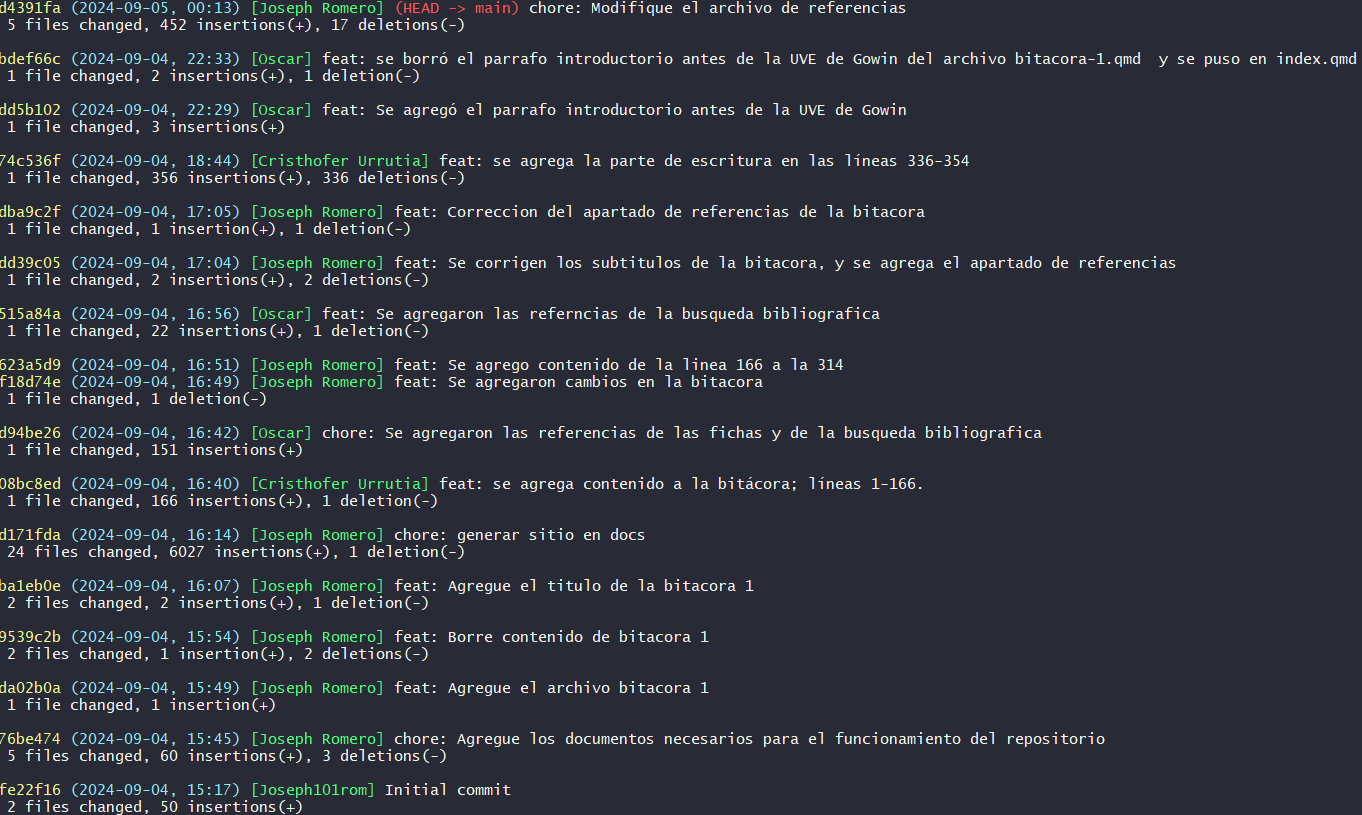
\includegraphics{imagenes/link-1.png}

}

\caption{Resultado del link}

\end{figure}%

\section{Comando 2:}\label{comando-2}

\begin{figure}[H]

{\centering 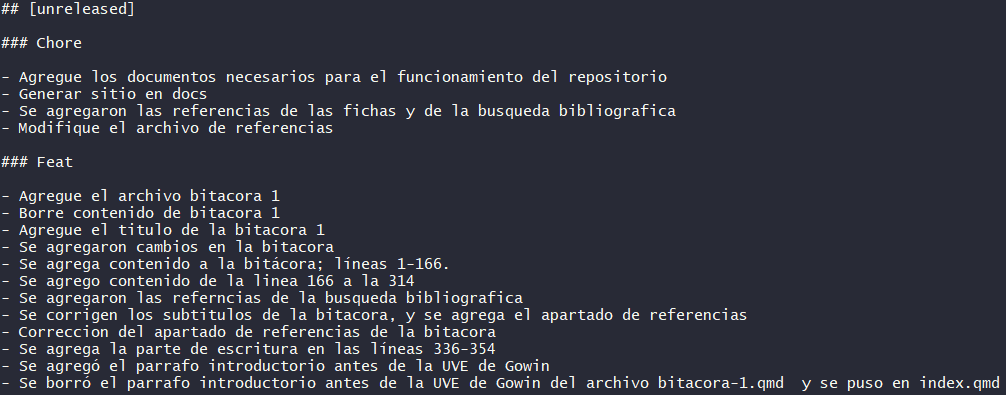
\includegraphics{imagenes/CHANGELOG-1.png}

}

\caption{Changelog}

\end{figure}%

\section{Comando 3:}\label{comando-3}

\begin{figure}[H]

{\centering 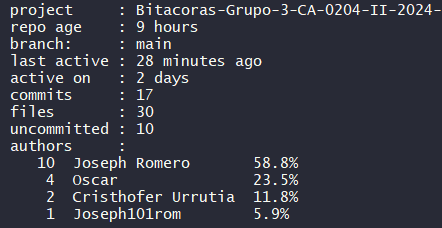
\includegraphics{imagenes/gitsummary-1.png}

}

\caption{Git summary}

\end{figure}%

\bookmarksetup{startatroot}

\chapter{Parte planificacion}\label{parte-planificacion}

\section{Pregunta de investigación:}\label{pregunta-de-investigaciuxf3n}

\subsection{Defincion del idea}\label{defincion-del-idea}

``Análisis del Éxito Comercial de Videojuegos Basado en Características
del Juego''

\subsection{Conceptualización de la
idea:}\label{conceptualizaciuxf3n-de-la-idea}

\begin{itemize}
\item
  Análisis: Por análisis se entiende el examen minucioso y pormenorizado
  de un asunto para conocer su naturaleza, sus características, su
  estado y los factores que intervienen en todo ello.
  \href{https://definicion.edu.lat/significados/analisis.html\#:~:text=Qu\%C3\%A9\%20es\%20An\%C3\%A1lisis\%3A\%20Por\%20an\%C3\%A1lisis\%20se\%20entiende\%20el,y\%20los\%20factores\%20que\%20intervienen\%20en\%20todo\%20ello.}{Fuente}
\item
  Éxito: El éxito es el resultado satisfactorio de una acción o
  proyecto.
  \href{https://definicion.edu.lat/concepto/exito.html}{Fuente}
\item
  Comercial: Comercial es un adjetivo que se refiere a lo vinculado con
  el comercio o con las personas que se dedican a comprar y/o vender
  bienes o servicios. El término comercio, por su parte, puede hacer
  mención a esta actividad o al espacio físico donde se desarrolla.
  \href{https://definicion.edu.lat/definicion/comercial.html}{Fuente}
\item
  Videojuegos: Los videojuegos son softwares de juegos electrónicos
  desarrollados para el entretenimiento a través de un aparato
  electrónico como máquinas arcade, consolas, computadores o
  dispositivos digitales.
  \href{https://definicion.edu.lat/significados/videojuego.html}{Fuente}
\item
  Basado: La palabra ``basado'' es el participio del verbo ``basar'' y
  se utiliza como un adjetivo para describir algo que se ha fundamentado
  o apoyado en una base específica.
  \href{https://www.definiciones-de.com/Definicion/de/basado.php\#:~:text=Definici\%C3\%B3n\%20de\%20basado\%20p.\%20La\%20palabra\%20\%22basado\%22\%20es,base\%20determinada\%2C\%20sin\%20perder\%20completamente\%20su\%20naturaleza\%20verbal.}{Fuente}
\item
  Característica: Las características de un objeto, una persona o un
  referente cualquiera son aquellos rasgos, condiciones o elementos que
  le resultan propios, reconocibles y que sirven para distinguirlo de
  otros referentes similares. Así, por ejemplo, las características de
  un perro incluyen su color, su tamaño, su raza, su conducta, su edad y
  todo aquello que nos sirva para distinguirlo del resto de los
  animales.
  \href{https://definicion.edu.lat/concepto/caracteristica.html}{Fuente}
\item
  Juego: Ejercicio recreativo o de competición sometido a reglas, y en
  el cual se gana o se pierde. \href{https://dle.rae.es/juego}{Fuente}
\end{itemize}

\subsection{Identificación de
tensiones:}\label{identificaciuxf3n-de-tensiones}

Definición de Variables y Métricas: Consideramos fundamental definir
correctamente las variables y las métricas de manera clara y concisa, ya
que en caso de no hacerlo puede resultar en una labor mucho más extensa
y complicada de lo esperado.

Selección de Técnicas de Análisis: En caso de no realizar una correcta
selección de técnicas de análisis, podríamos enfrentarnos ante un
proceso más largo y complicado de lo que debería de ser, además de no
brindar información fidedigna al analizar los datos con una técnica
inadecuada.

Definición de ``Éxito Comercial'': Pensamos que establecer una métrica
clara y consistente para medir el éxito comercial de los videojuegos
puede representar todo un desafío, pues este es un concepto que puede
depender de factores como ventas, popularidad e ingresos, lo que lo
vuelve un poco más complicado el ``limitar'' a la hora de definirlo.

Identificación de Características Clave del Juego: En caso de no escoger
las características de videojuegos adecuadas, puede que estas no estén
presentes en nuestra base de datos o que no nos lleven a conclusiones
relevantes, por ende afectando la integridad del proyecto.

Complejidad de las Relaciones: Entender las relaciones que pueden o no
darse entre las características del juego y el éxito comercial puede ser
algo complicado, pues existen interacciones y efectos que no son
precisamente lineales y que podrían requerir de técnicas de análisis
avanzadas (de las cuales no disponemos en este curso), lo que añade una
capa más de complejidad a nuestro estudio que no fué contemplada al
inicio.

Comparabilidad entre Juegos: Los videojuegos pueden diferir
significativamente en términos de presupuesto, marketing y otros
factores externos al juego en sí, lo cual puede hacer más difícil aislar
el efecto de las características de cada juego en el éxito comercial y
por ende dificultarnos la labor de llegar a concluir alguna relación
entre el juego y las características que lo llevaron ser exitoso.

\subsection{Reformulación de la idea en modo
pregunta}\label{reformulaciuxf3n-de-la-idea-en-modo-pregunta}

\begin{itemize}
\item
  ¿Cómo se puede analizar el mercado de los videojuegos?
\item
  ¿Por qué es importante analizar el mercado de los videojuegos para
  reconocer desencadenantes del éxito de la industria?
\item
  ¿Qué características son fundamentales para el éxito comercial de un
  videojuego dado el contexto donde fue publicado?
\item
  ¿Por qué a las personas les atraen los videojuegos y cuál es su
  relación con el éxito comercial de los videojuegos?
\end{itemize}

\subsection{Argumentación de la
preguntas:}\label{argumentaciuxf3n-de-la-preguntas}

¿Cómo se puede analizar el mercado de los videojuegos?

\emph{Contrargumentos:}

\begin{itemize}
\item
  \emph{Lógica:} El análisis podría ser limitado si se considerara un
  subanálisis predictivo. Esto debido a que el mercado puede dar giros
  radicales; por ejemplo, se puede dar el caso de que anuncien una nueva
  consola de videojuegos.
\item
  \emph{Ética:} Existen videojuegos cuya temática es la violencia y
  realizar un proyecto donde se mencionan dichos videojuegos podría
  conducir a una publicidad accidental de un mercado de juegos
  violentos.
\item
  \emph{Emocional:} Un análisis simplificado del mercado de los
  videojuegos puede omitir aspectos como la propia perspectiva de un
  consumidor frente a cierto tipo de videojuegos, por ejemplo.
\end{itemize}

\emph{Argumentos:}

\begin{itemize}
\item
  \emph{Lógica:} El análisis de este mercado podría aprovecharse de
  herramientas microeconómicas y macroeconómicas, pues a fin de cuentas
  sigue siguiendo un mercado.
\item
  \emph{Ética:} La mayoría de videojuegos requieren conexión permanente
  a internet, además, plataformas de videojuegos oficiales como Steam
  permiten acceder a bases de datos sobre videojugadores. Por lo tanto
  la información obtenida probablemente esté inalterada.
\item
  \emph{Emocional:} Gracias a los datos se podría ver que tan rentable
  es la industria de los videojuegos y de esta manera informar a la
  gente sobre dicha conclusión, pues existen muchas personas
  desempleadas que podrían incorporarse al mercado.
\end{itemize}

\emph{Conclusión:} El mercado de los videojuegos, como cualquier otro,
presenta sus propias problemáticas micro y macroeconómicas. Es gracias a
la salvedad de las herramientas económicas que se podrá hacer un
análisis desde ambas perspectivas (consumidor y empresas), sin embargo
se tendría un rezago en la parte emocional de las preferencias, por lo
que el análisis puede llegar a ser considerado tosco.

¿Por qué es importante analizar el mercado de los videojuegos para
reconocer desencadenantes del éxito de la industria?

\emph{Contrargumentos:}

\begin{itemize}
\item
  \emph{Lógica:} Existen otros mercados cuya influencia trasciende
  sustancialmente al de los videojuegos, un ejemplo de estos mercados
  puede ser el del petróleo, pues muchas actividades del día a día
  dependen de dicho recurso.
\item
  \emph{Ética:} En los últimos años se ha generado una gran ola de
  denuncias por parte de los trabajadores hacía las compañías
  desarrolladoras de videojuegos, lamentablemente, existen países como
  Japón en donde por su cultura los trabajadores no suelen visibilizar
  las problemáticas en los ambientes laborales. Por esta razón, la
  importancia de analizar este mercado no podría estar tan bien
  conceptualizada en este tipo de países. También podría darse el caso
  de que ciertos datos estén mostrando información ``falsa'', pues si se
  quisiera analizar las horas jugadas por jugador para asociar esto con
  las ventas, habría que tener en cuenta que muchas de esas horas
  corresponden a gente que estaba \emph{afk}.
\item
  \emph{Emocional:} La preferencia de los consumidores estarían
  respaldadas bajo datos estadísticos; lo que implica que se ignorarán
  experiencias que los jugadores hayan experimentado mientras jugaban.
\end{itemize}

\emph{Argumentos:}

\begin{itemize}
\item
  \emph{Lógica:} A nivel cultural sería interesante sonsacar la
  importancia de este mercado. Como expresión artística, los videojuegos
  podrían indicar una respuesta social a ciertos fenómenos de la
  actualidad como ha pasado con la música. Los datos estadísticos
  ayudarían a esclarecer este suceso.
\item
  \emph{Ética:} Un país en desarrollo como Costa Rica podría tomar
  acción al incursionar (o no) en el mercado de videojuegos gracias a
  las estadísticas. Si un país lograra éxito en este mercado sería
  posible aumentar las fuentes de ingresos.
\item
  \emph{Emocional:} Para muchas personas los videojuegos se les
  presentaron en su infancia; sería de especial interés conocer qué
  empresas han permanecido con sus sagas longevas de videojuegos y de
  esta manera complacer a sus consumidores.
\end{itemize}

\emph{Conclusión:} Pese a que bajo ciertas medidas los videojuegos no
sean una industria tan influyente, siempre existirá este mercado de
nicho que se mueve principalmente por razones emocionales. También es
importante recalcar irregularidades del mercado para que se puedan
corregir en el futuro y de esta manera mejorar el ambiente laboral, por
ejemplo. También, aunque parezca utópico por la naturaleza del tema: el
análisis puede servir para que gobiernos decidan si invertir recursos en
la industria.

¿Qué características son fundamentales para el éxito comercial de un
videojuego dado el contexto donde fue publicado?

\emph{Contrargumentos:}

\begin{itemize}
\item
  \emph{Lógica}: Los resultados de este análisis podrían no ser
  concretos. Los videojuegos empezaron a ser más notorios en la década
  de los 70 y desde entonces las tendencias han cambiado radicalmente.
\item
  \emph{Ética:} Si se fija el análisis dentro de un período específico,
  se obtendrían datos sobre características propias de videojuegos
  violentos, un ejemplo de esto es la década 2010-2020. De esta manera,
  se puede dar el caso de que algún grupo de personas interpreten de
  manera errónea la información.
\item
  \emph{Emocional:} Existen datos no parametrizables que pueden
  determinar el éxito de un videojuego, por ejemplo: la relación que
  pueden entablar varias personas en los juegos en línea.
\end{itemize}

\emph{Argumentos:}

\begin{itemize}
\item
  \emph{Lógica:} Sería posible tener un análisis que demuestre el
  panorama actual de las preferencias de los videojugadores, por lo que
  a nivel sociológico o cultural se podrían notar patrones en las
  características de los videojuegos. Por ejemplo, una característica
  que sería de gran ayuda para este propósito es la de ``géneros de los
  videojuegos''.
\item
  \emph{Ética:} Gracias a las características notadas, se podrían
  realizar sugerencias acerca de cómo tendrían que ser los videojuegos
  para mantener al público satisfecho.
\item
  \emph{Emocional:} El nicho de los videojuegos tiene una característica
  muy importante: la sociabilidad entre sus miembros. Realizar este
  análisis permitiría que las personas conozcan más acerca de sus
  preferencias en videojuegos y se vean incentivadas a socializar más.
\end{itemize}

\emph{Conclusión:} Aunque las características sean cambiantes, vale la
pena realizar un análisis sobre períodos fijos y de esta manera conocer
cuáles características fueron prevalecientes en dichos períodos. Un
punto bueno de este análisis es el de la posibilidad de notar las
mejores características de cada época y combinarlas para tratar de
combatir irregularidades del presente.

¿Por qué a las personas les atraen los videojuegos y su relación con el
éxito de la industria?

\emph{Contraargumentos:}

\begin{itemize}
\item
  \emph{Lógica:} Esta pregunta tiene una fuerte connotación emocional.
  Por lo tanto, resulta difícil socavar la premisa mediante datos
  numéricos y categóricos sencillos.
\item
  \emph{Ética:} Se ha visto casos de criminales que usan como medio a
  los videojuegos para realizar sus actos infames. Esto sucede gracias a
  juegos en línea en donde por ejemplo, un extorsionador puede utilizar
  a un infante para sus propósitos, por este y muchos otros motivos los
  videojuegos son atractivos para la delincuencia y los datos serían
  imprecisos para notarlo.
\item
  \emph{Emocional:} La atracción a los videojuegos puede conducir a una
  posterior adicción a los videojuegos, lo que repercute en
  consecuencias sociales negativas para el ya paciente psiquiátrico
  afectado. Desgraciadamente, la incorporación de este trastorno al
  DSM-V fue reciente por lo que no se tienen suficientes datos de este
  tema.
\end{itemize}

\emph{Argumentos:}

\begin{itemize}
\item
  \emph{Lógica:} No podemos hablar de éxito de los videojuegos (a un
  nivel más profundo) basados en sus características sin antes responder
  a esta interrogante, pues es de la respuesta que obtenemos en una
  versión más primitiva (pero al mismo tiempo madura) una lista de las
  tan ansiadas características asociadas a dicho éxito desde el punto de
  vista del videojugador.
\item
  \emph{Ética:} Es menester de la sociedad conocer a través de un
  análisis los patrones de conducta que llevaron al auge y vigencia este
  fenómeno. De este modo la población en general tendrá un mejor juicio
  y panorama acerca del tema.
\item
  \emph{Emocional:} Un mundo sin videojuegos sería inimaginable para
  muchas personas, al final de cuentas muchas personas utilizan a los
  videojuegos como una herramienta para escapar de su realidad. Conocer
  qué factores están anudados a esta ``fuga'' de realidad podría ayudar
  a las personas a buscar ayuda psicológica y/o mejorarla.
\end{itemize}

\emph{Conclusión:} El punto más débil es la falta de información que
pueden tener ciertos indicadores numéricos y categóricos para abstraer
esta pregunta y responder. Sin embargo, se podría solventar ese problema
al investigar de manera un poco más profunda sobre la conducta humana y
estadísticas que se usen en estudios con propósito similar.

\subsection{Argumentacion a traves de
datos.}\label{argumentacion-a-traves-de-datos.}

\emph{Fuente de Información:} La base de datos utilizada es el Steam
Games Dataset, recopilado por Martin Bustos Roman en 2022 y disponible
en Kaggle. Este dataset incluye información detallada sobre más de
85,000 videojuegos publicados en la plataforma Steam. El enlace de
acceso es: https://doi.org/10.34740/KAGGLE/DS/2109585.

\emph{Contexto Temporal y Espacial de los Datos:} Temporal: El dataset
cubre videojuegos lanzados desde los inicios de Steam hasta el año 2022,
lo que permite analizar la evolución del mercado de videojuegos durante
un período largo. Espacial: El dataset abarca un contexto espacial
mundial, lo que permite realizar análisis que reflejen las tendencias y
características del mercado de videojuegos a nivel internacional.

\emph{Facilidad de Obtener la Información:} La base de datos es de
acceso público a través de Kaggle, lo que facilita la obtención y uso de
la información. La recopilación de datos fue realizada utilizando la API
de Steam, complementada con datos de Steam Spy.

\emph{Población de Estudio:} La población de estudio incluye todos los
videojuegos disponibles en Steam, lo que representa una cobertura
extensa del mercado de videojuegos .

\emph{Muestra Observada:} La muestra observada consta de más de 85,000
videojuegos, proporcionando una base sólida y representativa para el
análisis.

\emph{Unidad Estadística o Individuos:} Cada unidad estadística en la
tabla representa un videojuego individual. Cada fila en la tabla
corresponde a un juego específico con sus características particulares,
como precio, fecha de lanzamiento, reseñas, entre otros.

\textbf{Descripción de las Variables de la Tabla}

\begin{itemize}
\tightlist
\item
  \textbf{AppID:} Identificador único del juego en Steam.
\item
  \textbf{Name:} Nombre del juego.
\item
  \textbf{Release date:} Fecha de lanzamiento del juego.
\item
  \textbf{Estimated owners:} Número estimado de propietarios del juego.
\item
  \textbf{Peak CCU:} Máximo número de usuarios concurrentes.
\item
  \textbf{Required age:} Edad mínima requerida para jugar el juego.
\item
  \textbf{Price:} Precio del juego en dólares estadounidenses.
\item
  \textbf{DLC count:} Número de contenidos descargables (DLC)
  disponibles para el juego.
\item
  \textbf{About the game:} Descripción breve del juego.
\item
  \textbf{Supported languages:} Idiomas soportados por el juego.
\item
  \textbf{Full audio languages:} Idiomas con soporte de audio completo.
\item
  \textbf{Reviews:} Reseñas de los usuarios.
\item
  \textbf{Header image:} URL de la imagen de encabezado del juego en la
  tienda.
\item
  \textbf{Website:} Sitio web oficial del juego.
\item
  \textbf{Support url:} URL de soporte del juego.
\item
  \textbf{Support email:} Correo electrónico de soporte.
\item
  \textbf{Windows:} Indica si el juego es compatible con Windows.
\item
  \textbf{Mac:} Indica si el juego es compatible con Mac.
\item
  \textbf{Linux:} Indica si el juego es compatible con Linux.
\item
  \textbf{Metacritic score:} Puntaje del juego en Metacritic.
\item
  \textbf{Metacritic url:} URL del juego en Metacritic.
\item
  \textbf{User score:} Puntaje otorgado por los usuarios.
\item
  \textbf{Positive:} Número de reseñas positivas.
\item
  \textbf{Negative:} Número de reseñas negativas.
\item
  \textbf{Score rank:} Clasificación del juego según el puntaje.
\item
  \textbf{Achievements:} Número de logros disponibles en el juego.
\item
  \textbf{Recommendations:} Número de recomendaciones del juego.
\item
  \textbf{Notes:} Notas adicionales sobre el juego.
\item
  \textbf{Average playtime forever:} Tiempo promedio de juego total.
\item
  \textbf{Average playtime two weeks:} Tiempo promedio de juego en las
  últimas dos semanas.
\item
  \textbf{Median playtime forever:} Mediana del tiempo de juego total.
\item
  \textbf{Median playtime two weeks:} Mediana del tiempo de juego en las
  últimas dos semanas.
\item
  \textbf{Developers:} Desarrolladores del juego.
\item
  \textbf{Publishers:} Publicadores del juego.
\item
  \textbf{Categories:} Categorías a las que pertenece el juego.
\item
  \textbf{Genres:} Géneros del juego.
\item
  \textbf{Tags:} Etiquetas descriptivas del juego.
\item
  \textbf{Screenshots:} URL de las capturas de pantalla del juego.
\item
  \textbf{Movies:} URL de los videos o tráilers del juego.
\end{itemize}

\textbf{Descripción Detallada de Elementos Clave:} Cada fila representa
un videojuego específico. En ellas se agrupan todos los atributos del
juego en cuestión, permitiendo comparaciones entre diferentes juegos y
análisis de cómo sus características contribuyen a su éxito.Además las
columnas representan las características específicas de cada videojuego,
como su precio, número de reseñas positivas y su puntaje en Metacritic.
Estas columnas son esenciales para analizar cómo diferentes factores
influyen en el éxito comercial de un Juego. Por otro lado las celdas
contienen los valores específicos de cada variable para cada juego.
Estas celdas permiten realizar un análisis granular, observando cómo
cada característica afecta el éxito de un videojuego.

\textbf{Relación con la Pregunta de Investigación:} La diversidad de
datos (como fecha de lanzamiento, precio y popularidad) permite un
análisis profundo del mercado de videojuegos, observando tendencias a lo
largo del tiempo.La información sobre la cantidad de juegos, sus
características y el comportamiento del consumidor es crucial para
entender la dinámica del mercado. Por otra parte, variables como
``Metacritic score,'' ``User score,'' y ``Estimated owners'' son
fundamentales para determinar qué características son más influyentes en
el éxito comercial de los videojuego.

\section{Revisión bibliográfica}\label{revisiuxf3n-bibliogruxe1fica}

\subsection{Búsqueda de
bibliografía}\label{buxfasqueda-de-bibliografuxeda}

\begin{itemize}
\tightlist
\item
  Somos Xbox (2024)
\item
  El Periódico (2019)
\item
  Desconocido (2024a)
\item
  We Are Testers (2024)
\item
  Desconocido (2024c)
\item
  AppsFlyer (2024)
\item
  Desconocido (2023a)
\item
  Puro Marketing (2023)
\item
  Desconocido (2023b)
\item
  Desconocido (2021)
\item
  Desconocido (2024b)
\end{itemize}

\subsection{Construcción de fichas de
literatura}\label{construcciuxf3n-de-fichas-de-literatura}

\textbf{Ficha 1:}

\textbf{■ Título:} Manga, anime y videojuegos japoneses: análisis de los
principales factores de su éxito global

\textbf{■ Autor(es):} Carmen Mangirón

\textbf{■ Año: 2012}

\textbf{■ Nombre del tema:} Estrategias de globalización en la cultura
japonesa.

\textbf{■ Forma de organizarlo:}

\begin{itemize}
\item
  \textbf{Cronológico:} Desde la crisis económica de Japón en los años
  90.
\item
  \textbf{Metodológico:} Análisis de mercado y estrategias de marketing.
\item
  \textbf{Temático:} Análisis transmediático.
\item
  \textbf{Teoría:} Cool Japan.
\end{itemize}

\textbf{■ Resumen en una oración:} Se analizan las estrategias de
globalización de la cultura popular japonesa.

\textbf{■ Argumento central:} Las empresas japonesas han adoptado
estrategias efectivas para internacionalizar sus productos culturales.

\textbf{■ Problemas con el argumento o el tema:} La traducción es un
reto con el que el autor ha tenido que lidiar.

\textbf{■ Resumen en un párrafo:} En esta obra el autor explica cómo
algunas expresiones de arte de la cultura japonesa como lo son el manga,
el anime y los videojuegos han logrado una expansión internacional muy
significativa desde la década de 1990. Trata temas como las estrategias
de globalización que ayudaron a que las empresas japonesas lleguen a los
mercados de todo el mundo, también se mencionan algunos fenómenos como
lo puede ser la traducción no oficial hecha por aficionados. A pesar del
éxito de estas empresas el autor menciona que ha sido un gran reto para
las empresas japonesas lograr que sus productos sean aceptados del todo
en los mercados extranjeros debido a las diferencias culturales.

\textbf{■
\href{https://funderetica.org/wp-content/uploads/2017/01/Cuaderno-7-web-def.pdf}{Fuente}}:Hevia
(2012)

\textbf{Ficha 2:}

\textbf{■ Título:} Problematic video game use as an emotional coping
strategy: Evidence from a sample of MMORPG gamers

\textbf{■ Autor(es):} Maria Di Blasi

\textbf{■ Nombre del tema:} Gaming Disorder

\textbf{■ Forma de organizarlo:}

\begin{itemize}
\item
  \textbf{Cronológico:} Se ubicó entre el año 2017 y 2018.
\item
  \textbf{Metodológico:} Encuestas y datos estadísticos.
\item
  \textbf{Temático:} Datos asociados a la salud mental de los jugadores.
\item
  \textbf{Teoría:} Los videojuegos como método para escapar de la
  realidad.
\end{itemize}

\textbf{■ Resumen en una oración:} Se analizó el comportamiento de los
jugadores encuestados y se relacionó a la desregularización emocional.

\textbf{■ Argumento central:} La fuerte relación del estado emocional y
los videojuegos.

\textbf{■ Problemas con el argumento o el tema:} El autor a veces puede
llegar a sonar redundante.

\textbf{■ Resumen en un párrafo:} Los videojuegos, como cualquier otro
medio de entretenimiento genera placer. El problema de generar placer es
que muchas personas pueden llegar a entretenerse de esta manera para
compensar estados emocionales irregulares y que a la larga en vez de
obtener beneficios se obtengan desventajas. La muestra fueron jugadores
de un juego en línea llamado World of Warcraft: en este juego se reportó
una gran satisfacción por parte de los encuestados, sin embargo también
se notó que muchos llegaban a estresarse bastante durante sus sesiones
de juego.

\textbf{■
\href{https://www.ncbi.nlm.nih.gov/pmc/articles/PMC7044601/}{Fuente}}

\textbf{Ficha 3:}

\textbf{■ Título:} ¿Qué hace un videojuego divertido?

\textbf{■ Autor(es):} Guerrero Pastor, Marta

\textbf{■ Año:} 2023

\textbf{■ Nombre del tema:} Elementos que contribuyen a la diversión en
los videojuegos.

\textbf{■ Forma de organizarlo:}

\begin{itemize}
\item
  \textbf{Cronológico:} El estudio se contextualiza en el marco de
  teorías y prácticas actuales sobre el diseño de videojuegos.
\item
  \textbf{Metodológico:} Investigación teórica seguida de encuestas
  realizadas a jugadores.
\item
  \textbf{Temático:} Elementos que influyen en la diversión durante el
  diseño de videojuegos.
\item
  \textbf{Teoría:} Psicología de la diversión aplicada al diseño de
  videojuegos.
\end{itemize}

\textbf{■ Resumen en una oración:} Este estudio investiga los
componentes clave que hacen que un videojuego sea divertido desde una
perspectiva teórica y práctica.

\textbf{■ Argumento central:} La diversión en los videojuegos se
descompone en múltiples factores como el aprendizaje, la experiencia del
jugador y la interacción social, todos los cuales son cruciales para una
experiencia de juego atractiva.

\textbf{■ Problemas con el argumento o el tema:} El desafío de capturar
todos los aspectos que contribuyen a la diversión en un solo estudio,
señalando la necesidad de más investigaciones en áreas menos exploradas.

\textbf{■ Resumen en un párrafo:} Se exploran los elementos que hacen
que un videojuego sea divertido, y se va dividiendo la investigación en
tres fases: revisión teórica, encuestas y análisis de resultados. Se
identifican factores clave como el aprendizaje, la variedad y la
interacción social como fundamentales para mantener el interés del
jugador. El estudio reconoce la necesidad de explorar más áreas de la
diversión en videojuegos, sugiriendo que los resultados obtenidos abren
nuevas preguntas sobre la naturaleza de esta diversión.

\textbf{■ Fuente:} Guerrero Pastor (2018)

\section{Construcción de la UVE de
Gowin}\label{construcciuxf3n-de-la-uve-de-gowin}

\begin{figure}[H]

{\centering 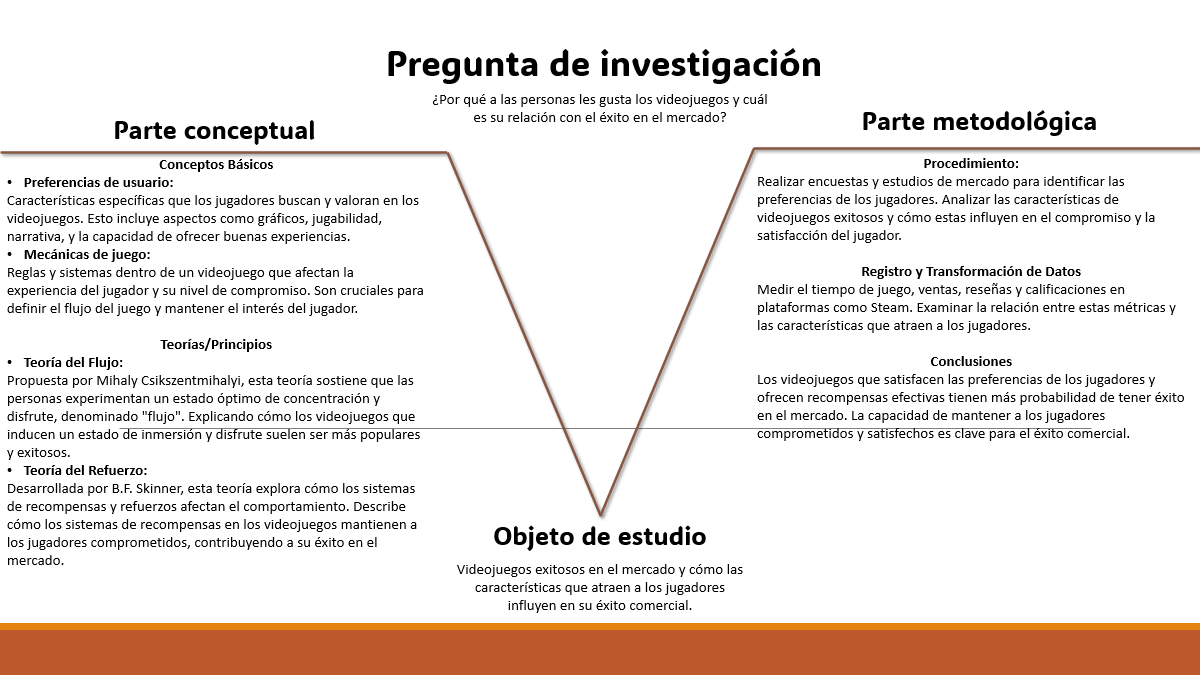
\includegraphics{imagenes/V-de-gowin.png}

}

\caption{Diagrama de Gowin}

\end{figure}%

Fuentes:

\begin{itemize}
\item
  Csikszentmihalyi (1990)
\item
  Skinner (1938)
\end{itemize}

\bookmarksetup{startatroot}

\chapter{Parte de escritura}\label{parte-de-escritura}

\section{Selección de la pregunta:}\label{selecciuxf3n-de-la-pregunta}

¿Por qué a las personas les atraen los videojuegos y cuál es su relación
con el éxitocomercial de los videojuegos?

\subsection{Argumentación:}\label{argumentaciuxf3n}

La pregunta escogida tiene origen en la investigación realizada de las
otras tres preguntas potenciales. La razón principal es qué la misma
tiene la característica de englobar (no necesariamente en una magnitud
uniforrme) a las demás de manera explícita como ímplicita. Para
dilucidar la naturaleza de la pregunta, se mostrará la siguiente
comparación:

\textbf{(i)} ¿Qué características son fundamentales para el éxito
comercial de un videojuego dado el contexto donde fue publicado? ó ¿Por
qué a las personas les atraen los videojuegos y cuál es su relación con
el éxitocomercial de los videojuegos?

Primero, note que el corazón de la primera pregunta reside en las
palabras \emph{características} y \emph{fundamentales}. De esta
pregunta, podemos plantear las siguientes: ¿Existen características
generales que hagan que a las personas les gusten los videojuegos? y ¿Si
existen dichas características, qué tan fundamentales son en el mercado
de los videojuegos para la desición de los consumidores? Se puede
hallar, de manera parcial, una respuesta a ambas preguntas en el
escapismo que menciona Di Blasi (2019) en su respectivo artículo; pero
es que además esta respuesta funge de igual manera en la pregunta
elegida por el grupo. Finalmente, tras confrontar ambas preguntas y
notar esta relación: se determinó cuál pregunta resultó vencedora, o sea
la que se eligió.

\textbf{(ii)} ¿Por qué es importante analizar el mercado de los
videojuegos para reconocer desencadenantes del éxito de la industria? ó
¿Por qué a las personas les atraen los videojuegos y cuál es su relación
con el éxitocomercial de los videojuegos?

El vínculo entre estas dos preguntas no parece tan clara a primera
vista, no obstante y de manera empírica se pueden utilizar las
conclusiones del Estudio sobre juegos para móviles: hábitos en el sector
`gaming' (We Are Testers (2024)) para proponer respuestas a la primera
pregunta. En este estudio se mencionan dos cosas importantes:
\emph{frecuencia de juego} y \emph{celulares}, el celular es
posiblemente el objeto más utilizado del siglo ventiúno. ``El celular es
el objeto más utilizado'' es lo mismo que decir ``La frecuencia de uso
del celular corresponde a la mayor de otro objeto'', entonces es natural
pensar que si existen videojuegos de celulares, esto implicaría que no
es de extrañar que los videojuegos para móbiles sean tan populares; ¿Son
estas características fundamentales (relación con lo planteado en (i))
para el éxito de los videojuegos? Si la respuesta es afirmativa,
entonces por transitividad se llega a que esta podría ser una razón de
preferencia de los consumidores frente a los videojuegos. De semejante
manera se llega a la misma conclusión que en (i): la respuesta ante la
hipótesis planteada en este inciso funciona para ambas interrogantes.

\textbf{(iii)} ¿Cómo se puede analizar el mercado de los videojuegos? ó
¿Por qué a las personas les atraen los videojuegos y cuál es su relación
con el éxito comercial de los videojuegos?

Se desestimó fácilmente la primera pregunta, pues el mercado se puede
analizar desde las preferencias, y para entender las preferencias se
necesita entender el por qué de esta; o sea, el origen de la atracción
que los videojuegos han cultivado en millones de personas. \#

\bookmarksetup{startatroot}

\chapter*{Referencias:}\label{referencias}
\addcontentsline{toc}{chapter}{Referencias:}

\phantomsection\label{refs}
\begin{CSLReferences}{1}{0}
\bibitem[\citeproctext]{ref-Ref6}
AppsFlyer, Equipo de. 2024. {«Análisis de juegos: Por qué importan los
números»}. \emph{AppsFlyer}.
\url{https://www.appsflyer.com/es/blog/measurement-analytics/gaming-analytics/}.

\bibitem[\citeproctext]{ref-V1}
Csikszentmihalyi, Mihaly. 1990. \emph{Flow: The Psychology of Optimal
Experience}. Harper \& Row.

\bibitem[\citeproctext]{ref-Ref10}
Desconocido, Autor. 2021. {«Análisis de datos para mejorar el diseño de
videojuegos»}. \emph{Gamasutra}.
\url{https://www.gamasutra.com/view/news/365991/Using_data_to_improve_game_design_A_case_study.php}.

\bibitem[\citeproctext]{ref-Ref7}
---------. 2023a. {«Cómo hacer un análisis de mercado para un
videojuego»}. \emph{YouTube}.
\url{https://www.youtube.com/watch?v=zQFRMqSBxtY}.

\bibitem[\citeproctext]{ref-Ref9}
---------. 2023b. {«Éxito Igual a Adaptación al Cliente en la Industria
del Videojuego»}. \emph{Grafiati}.
\url{https://www.grafiati.com/en/blogs/how-to-cite-a-video-game/}.

\bibitem[\citeproctext]{ref-Ref3}
---------. 2024a. {«Análisis de la industria del videojuego en España»}.
\emph{Riunet}.
\url{https://riunet.upv.es/bitstream/handle/10251/45702/Trabajo\%20final\%20carrera.pdf}.

\bibitem[\citeproctext]{ref-Ref11}
---------. 2024b. {«Cómo medir el éxito de un videojuego»}. \emph{Pocket
Gamer}.
\url{https://www.pocketgamer.biz/comment-and-opinion/77568/how-to-measure-the-success-of-your-game/}.

\bibitem[\citeproctext]{ref-Ref5}
---------. 2024c. {«Plan de marketing para una empresa de videojuegos»}.
\emph{Universidad Nacional de Cuyo}.
\url{https://bdigital.uncu.edu.ar/objetos_digitales/15654/plan-de-marketing-para-una-empresa-de-videojuegos.pdf}.

\bibitem[\citeproctext]{ref-maria2019}
Di Blasi, Maria. 2019. {«Problematic video game use as an emotional
coping strategy: Evidence from a sample of MMORPG gamers»}.
\emph{Journal of Behavioral Addictions} 8 (1): 25-34.
https://doi.org/\url{https://doi.org/10.1556/2006.8.2019.02}.

\bibitem[\citeproctext]{ref-Ref2}
El Periódico, Equipo de. 2019. {«Esta es la receta del éxito de los
videojuegos»}. \emph{El Periódico}.
\url{https://www.elperiodico.com/es/economia/20190704/exito-videojuegos-experiencia-usuario-7535607}.

\bibitem[\citeproctext]{ref-josephficha1}
Guerrero Pastor, Marta. 2018. {«?{}` Qu{é} hace divertido un videojuego?
Acercamiento al concepto de diversi{ó}n a trav{é}s del an{á}lisis de
videojuegos»}.

\bibitem[\citeproctext]{ref-Referencia-ficha-1}
Hevia, Carme Mangiron i. 2012. {«Manga, anime y videojuegos japoneses::
an{á}lisis de los principales factores de su {é}xito global»}.
\emph{Puertas a la lectura}, n.º 24: 28-43.

\bibitem[\citeproctext]{ref-Ref8}
Puro Marketing, Equipo de. 2023. {«Mentalidad de Jugadores y Publicidad
en Juegos Móviles»}. \emph{Puro Marketing}.
\url{https://www.puromarketing.com/21/212342/mentalidad-jugadores-clave-para-exito-publicidad-marcas-juegos-moviles}.

\bibitem[\citeproctext]{ref-V2}
Skinner, B. F. 1938. \emph{The Behavior of Organisms: An Experimental
Analysis}. Appleton-Century.

\bibitem[\citeproctext]{ref-Ref1}
Somos Xbox, Equipo de. 2024. {«Descifrando el éxito en el mundo de los
videojuegos. ¿Qué hace que un juego triunfe?»} \emph{Somos Xbox}.
\url{https://www.somosxbox.com/descifrando-el-exito-en-el-mundo-de-los-videojuegos-que-hace-que-un-juego-triunfe/}.

\bibitem[\citeproctext]{ref-Ref4}
We Are Testers, Equipo de. 2024. {«Estudio de mercado sobre juegos para
móviles y gaming»}. \emph{We Are Testers}.
\url{https://www.wearetesters.com/estudios-de-mercado/gaming/}.

\end{CSLReferences}



\end{document}
